\documentclass[bibtotoc,liststotoc,BCOR5mm,DIV12]{scrbook}

% use this declaration to set specific page margins
%\usepackage[a4paper , lmargin = {2.7cm} , rmargin = {2.9cm} , tmargin = {2.7cm} , bmargin = {4.6cm} ]{geometry}
\usepackage[a4paper]{geometry}
\usepackage{verbatim} 
\usepackage[ngerman, english]{babel}
\usepackage{bibgerm}       		% german references
%\usepackage[latin1]{inputenc} % german characters
\usepackage{graphicx} 				% it's recommended to use PDF images but you can use JPG or PNG as well
\usepackage{url}           		% format URLs
\usepackage{hyperref} 				% create hyperlinks
\usepackage{listings, color}	% for source code
\usepackage{subfig}						% two figures next to each other (example: figure 3a), figure 3b)
\usepackage{scrpage2}					% header and footer line
\usepackage{array}
\usepackage{pdfpages}
\newcolumntype{L}[1]{>{\raggedright\let\newline\\\arraybackslash\hspace{0pt}}m{#1}}
\newcolumntype{C}[1]{>{\centering\let\newline\\\arraybackslash\hspace{0pt}}m{#1}}
\newcolumntype{R}[1]{>{\raggedleft\let\newline\\\arraybackslash\hspace{0pt}}m{#1}}
% header and footer line - no header & footer line on pages where a new chapter starts
\pagestyle{scrheadings}
\ohead{Comparison of Spinoffs vs StartsUps in innovation capabilities}
\ofoot[]{\thepage}
\ifoot{I\&E Minor Thesis, Technische Universität Berlin, 31 Aug 2017}

% set path where images are stored
\graphicspath{{./img/}}

\begin{document}
% ---------------------------------------------------------------
\frontmatter
    \thispagestyle{empty}
\begin{center}

\vspace*{1.4cm}
{\LARGE \textbf{Technische Universit�t Berlin}}

\vspace{0.5cm}

{\large School of Economics and Management\\[1mm]}
{\large Centre for Entrepreneurship\\[5mm]}

Stra�e des 17. Juni 135\\
10623 Berlin\\
www.entrepreneurship.tu-berlin.de\\

\vspace*{1cm}


\includegraphics[width=4cm]{tu_logo.jpg}

\vspace*{1.0cm}

{\LARGE I\&E Minor Thesis}\\

\vspace{1.0cm}
{\LARGE \textbf{Comparison of Spinoffs vs }}\\
\vspace*{0.3cm}
{\LARGE \textbf{StartsUps in innovation capabilities}}\\
\vspace{0.3cm}
{\normalsize \textbf{Study of factors affecting innovation methods }}\\
\vspace*{0.3cm}
{\normalsize \textbf{of spinoffs and startups}}\\
\vspace*{1.0cm}
{\LARGE Amna Waseem}
\\
\vspace*{0.5cm}
Matriculation Number: 387424\\
01.01.2010\\ % 	date of submission
\vspace*{1.0cm}

Supervised by\\
Laura Helen Middermann\\
\vspace{3cm}


\end{center}


   	\thispagestyle{empty}
    \cleardoublepage
    
    \thispagestyle{empty}
\vspace*{1.0cm}

\begin{center}
    \textbf{Abstract}
\end{center}

\vspace*{0.5cm}

\noindent
In recent years, our lives have been drastically improved by revolutionary technologies and
innovations. This has been made possible by visions of entrepreneurs and leaders working in
businesses like spin-offs and start-ups. Both spin-offs and start-ups have been widely adopted in
entrepreneurial world and have been proven to be highly successful in terms of competitiveness,
innovativeness, growth, and economical development. However, there is still a gap in understanding the
major differences in innovation capabilities of spin-offs and start-ups. This research is focused
on finding the major factors which affect the innovation performance of start-ups
and spin-offs. Literary theories i.e. resource-based theory, human capital theory, social capital theory and motivational theory had been used in this paper
to find such factors and developed hypotheses which were tested using literature reviews and qualitative exploratory questionnaires. 
This study will help weave the path for future theoretical and experimental research on
comparing start-ups with spin-offs regarding innovation developments and help business owners to plan their innovative
strategies efficiently.
\\
\medskip

%\noindent \textit{JEL classification}: XXX, YYY.

\medskip
\noindent \textit{Keywords}: Startup, Spin-offs, Innovation Capabilities, Innovation Performance, Resource-based Theory, Human Capital Theory, Social Capital Theory, Motivational Theory
    \thispagestyle{empty}
    \cleardoublepage
    
    \tableofcontents
    \thispagestyle{empty}
    
    \listoffigures
    \thispagestyle{empty}
    
    \listoftables
    \thispagestyle{empty}
    
% --------------------------------------------------------------

\mainmatter % comment single chapters for faster compilation

    \chapter{Introduction\label{cha:chapter1}}

In this world of technological and innovation development, we have seen a continuous
evolution in types of businesses. Though the objective of each type of firm is same i.e. to generate
revenue by creating value for customers, there are differences in their approach to innovate and
maintain sustainability. Two types of businesses which have been the focus of attention to
entrepreneurs and researchers for many years are spin-offs and start-ups. Both businesses have contributed to
improve nation’s economies and employment rates. However, there are differences in their
innovation capabilities and their establishment processes.


\section{Motivation\label{sec:moti}}
In entrepreneurial literature, there have been several studies for understanding the taxonomy and formation of spin-off firms and start-ups.
Researchers have been trying to narrow the gap between theoretical understanding of processes adopted by spin-offs and start-ups and their related practical implications. Both businesses have been studied to understand their topologies, reasons of success and failures \cite{fastcompany}, and their affects on
the economical growth\cite{economical_growth}. There are also numerous comparative studies between spin-offs and
start-ups based on technological development \cite{comparative_studies}, resource inheritance and exploitation \cite{resource_inheritance}, and
survival and growth rate \cite{whose_child}. However, there has been little research on finding the major factors which
affect the innovation processes of start-ups and spin-offs.

\section{Objective\label{sec:objective}}
The purpose of this paper is to investigate major factors which affect the innovation methods of
spin-offs and start-ups. It has addressed this problem by reviewing existing literature and using
exploratory interviews with founders of spin-offs and start-ups. This study will guide the future research in this domain and facilitates business owners to
develop strategies for their business's success.


\section{Outline\label{sec:outline}}

The remainder of this paper is summarized as follows:
\\
In \textbf{Section \ref{cha:chapter2}}, prior research will be discussed
in order to lay foundations of the problem in hand.
\\
\\
Based on the theoretical discussion, \textbf{Section \ref{cha:chapter3}} will describe theoretical framework which will help to identify major factors for comparison and develop hypotheses. 
\\
\\
In \textbf{Section \ref{cha:chapter4}}, methodology of collecting data for testing hypotheses will be
discussed
\\
\\
\textbf{Section \ref{cha:chapter5}} will analyze the data and derive meaningful results.
\\
\\
Final \textbf{Section \ref{cha:chapter6}} concludes the research, discusses its potential benefits and identifies the opportunities for future
work.

    \chapter{Literature Review\label{cha:chapter2}}

This section explains the important definitions and previous research on start-ups and spin-offs to
gain better understanding of purpose of this research.

\section{Definitions of Start-Ups \label{sec:defs}}
According to \textbf{Wikipedia} \cite{6}:
``A startup company (startup or start-up) is an entrepreneurial venture which is typically a newly
emerged, fast-growing business that aims to meet a marketplace need by developing or offering an
innovative product, process or service.''
\\
\\
According to Steve Blank \cite{8}:
``A startup is a temporary organization designed to search for a repeatable and scalable business
model''.
\\
\\
``A startup is a company working to solve a problem where the solution is not obvious and success
is not guaranteed,'' says Neil Blumenthal, co-founder and co-CEO of Warby Parker \cite{9}.
\\
\\
TechCrunch writer Alex Wilhelm defines startup by ``50-100-500'' rule as follows:
``If your company has, or is any of the following, you have to hang up your Startup Uniform, and
realize that you are just another technology company either hunting for or actively avoiding an
IPO," Wilhelm writes. "\$50 million revenue run rate (forward 12 months); 100 or more
employees;Worth more than \$500 million, on paper or otherwise.'' \cite{10}
\\
\\
In a nutshell, there exists no single definition of start-up. Having read many definitions and views of
people about start-ups, I have come up with my own definition:
\\
\\
\textbf{``A start-up is an entrepreneurial venture aimed at creating value for itself and its customers by
solving a specific problem and embracing risks and failures on its way to become a stable business.
It is the outcome of efforts of individuals who work on their own resources without inheriting any
support from other organizations.''}
\\
\\

\newpage

\section{Definitions of Spin-Offs\label{sec:defs_spinoffs}}

According to \textbf{Wikipedia}\cite{7}:
\\
``Spin-offs are divisions of companies or organizations that then become independent businesses
with assets, employees, intellectual property, technology, or existing products that are taken from
the parent company.''
\\
\\
According to \textbf{Merriam Webster Dictionary} \cite{11}:
\\
``spin-off is the distribution by a business to its stockholders of particular assets and especially of
stock of another company; also: the new company created by such a distribution''
\\
\\
\textbf{The Economist Group Limited} published in blog ``\textbf{The art of the spin-off}'' \cite{12}:
\\
``In business, spin-offs are the offspring of established companies. You take a division and turn it
into a free-standing firm.''
\\
\\
A number of other studies define a spin-off as a firm whose intellectual capital originates in its
parent, for example, a university, research institute, or another companies \cite{13}.
The definition of spin-off varies depending upon the type of spin-off we are referring to. Broadly
speaking, there are two types of spin-offs i.e. Academic spin-offs and Corporate spin-offs. These
two types are further classified by researchers based on resource transfer, parental support and
reasons of their creation \cite{14}
\section{Previous Research on Start-Ups\label{sec:previous_r_startups}}
Research on Start-ups have been going on since 1980’s. The
relationship between innovativeness and success of firms has been the focus of research in literature
for many decades. Schumpeter \cite{16} described that innovativeness increased market power of a firm.
Porter \cite{17} explained that innovation improved the ability of firms to break competition. Zahra
and George \cite{18} had credited innovativeness for enhancing absorptive capacity of a company.
\\
\\
However, a lot of researchers also described negative affects of innovativeness. Samuelsson and
Davidsson \cite{19} stated that innovations could lead to introducing risks in success of start-ups.
Amason, Shrader and Tompson \cite{20} had declared innovativeness and novelty a great liability in the
path of start-ups’ success . John Freeman and Jerome S. Engel \cite{15} had compared start-ups with
corporate companies in their innovation models. According to them, big companies have
more capital, scientists and engineers, brand presence, strategic alliances, evolving organizational
structures, and well established business processes. On the other hand, young firms are a victim of
newness and are at higher risks of failure in the beginning. However, they have also mentioned that
big companies can fail in developing innovative products due to immobility in resources and
misalignment of incentives. In such scenarios, start-ups could evolve into sustainable, growing and
profitable businesses. Ari Hyytinen , Mika Pajarinen and Petri Rouvinen \cite{21} suggested that a
startup's innovativeness might in fact hurt its survival prospects. Their research has found that
survival rate for innovative startups is approximately 6–7 percentage points lower than that of non-
innovators. They also find that the interaction of innovativeness and entrepreneurs' greater appetite
for risk further reduces the prospects for survival.
\\
\\
In view of extensive research on finding affects of innovativeness on start-ups, it seems
that innovation might have either a positive or negative affect on start-ups’ success rate.
However, empirical literatures mostly states that results are positive \cite{21}.
\section{Previous Research on Spin-Offs\label{sec:previous_r_spin}}
No one can deny the importance of spin-offs in recent economic developments. Forbes calculates
that American companies completed more than 80 spin-offs worth at least \$500m each between
2002 and 2012 \cite{12}.There has been research on understanding corporate spin-offs topology \cite{23}. 
Helmut and Mike \cite{24} studied topology of spin-offs with respect to their environmental contexts as
shown in figure \ref{fig1} and defined four types of spin-offs i.e. Academic spin-off, Corporate spin-off,
Privatization buyout/buy-in of university research and Management buy-out/buy-in of division.

\begin{figure}[htb]
	\centering
	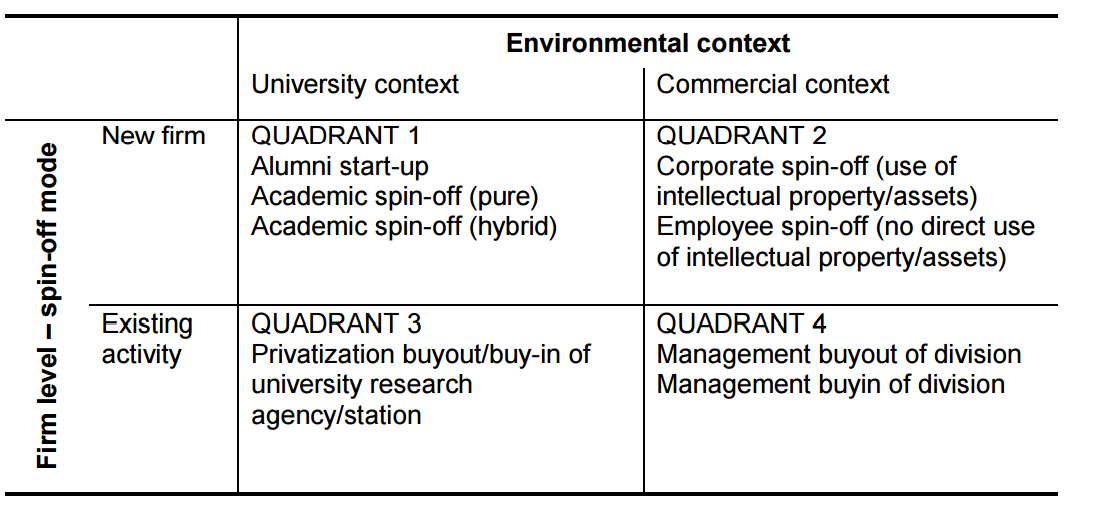
\includegraphics[width=10cm]{fig1}
	\caption{Topology of spin-offs. Adapted from ``The origin of spin-offs: a typology of corporate and academic spin-offs.'' by Fryges, Helmut, and Mike Wright. Small Business Economics 43.2 (2014)}
	\label{fig1}
\end{figure}

Sierdjan Koster did a survey of the founders of new companies and found that existing companies
had a positive impact on creation of new businesses and provides a basis for the new company to
build on. However, supported companies are less innovative \cite{50}.
\\
\\
In 1999, Institute for Prospective Technological Studies (IPTS) delivered a report ``The Impact of
Corporate Spin-Offs on Competitiveness and Employment in the European Union'' in which seven
countries were investigated ( United Kingdom, Sweden, Spain, Italy, Germany, France, and
Denmark ) based on two types of Corporate Spin-offs i.e. Restructuring-driven Spin-Off and
Entrepreneurial Spin-Offs \cite{26}. The results have shown that Corporate Spin-Off processes represent
a valuable mechanism for the transfer of technological and business knowledge and can produce
considerable impacts on competitiveness and the socio-economic environments. 
\\
\\
Andreas Stephan, in his research \cite{22}, compared research-based spin-offs with comparable knowledge-intensive firms
created in other ways. He found that out of 121 research spin-offs investigated have more patent
applications and more radical product innovations, on average, compared to similar firms.
Research has also been done in understanding the taxonomies of research-based spin-offs based on
type of resources, the business model and institutional links \cite{27}. Guido Buenstorf \cite{28} has compared
characteristics of spin-offs formed on basis of triggering events as necessity and opportunity spin-
offs. He described four types of useful knowledge which employees can learn in parent
companie i.e. knowledge about technology, markets and customer needs, organizational
processes, and personal skills.

\section{Previous Research on Comparison of Spin-Offs with Start-Ups\label{sec:previous_r_comparison}}
Peter and Viliam \cite{29} provided a theoretical framework for comparing start-ups and spin-offs in
terms of different types of support they need. James and Dennis \cite{31} had done research on different forms of incentives ,in form of property rights
and sufficient funds, faced by employees and employers which results in creation of either a start-up
or a spin-off.
Sierdjan Koster \cite{30} has compared start-ups and spin-offs based on resource theory using empirical
study of American entrepreneurs and showed that spin-offs are indeed a step ahead of firms that do
not receive support from a third party company. He identified four different types of firms based on
resource sharing and parental support as shown in figure \ref{fig2} .
\begin{figure}[htb]
	\centering
	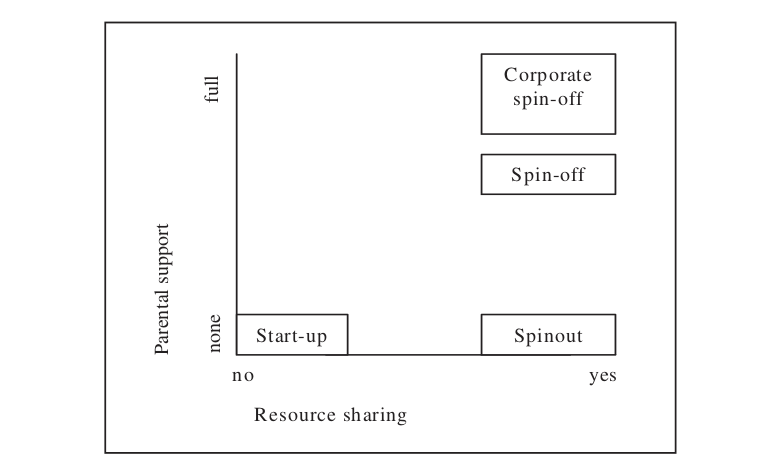
\includegraphics[width=8cm]{fig2}
	\caption{Difference between Start-up and spin-off based on resource and parental support. Adapted from ``Spin-off firms and individual start-ups. Are they really different?.'' by Sierdjan Koster. ERSA conference papers (2004)}
	\label{fig2}
\end{figure}

\begin{comment}

\begin{table}[htb]
\centering
\begin{tabular}[t]{|l|l|l|l|}
\hline
Name & Vendor & Release Year & Platform \\
\hline
\hline
A & Microsoft & 2000 & Windows \\
\hline
B & Yahoo! & 2003 & Windows, Mac OS \\
\hline
C & Apple & 2005 & Mac OS \\
\hline
D & Google & 2005 & Windows, Linux, Mac OS \\
\hline
\end{tabular}
\caption{Comparison of technologies}
\label{tab:enghistory}
\end{table}

\section{Standardization \label{sec:standard}}

This sections outlines standardization approaches regarding X.

\subsection{Internet Engineering Task Force\label{sec:itu}}

The IETF defines SIP as '...' \cite{rfcsip}

\subsection{International Telecommunication Union\label{sec:itu}}

Lorem Ipsum...

\subsection{3GPP\label{sec:3gpp}}

Lorem Ipsum...

\subsection{Open Mobile Alliance\label{sec:oma}}

Lorem Ipsum...

\section{Concurrent Approaches \label{sec:summ}}

There are lots of people who tried to implement Component X. The most relevant are ...
\end{comment}
    \chapter{Theoretical Framework\label{cha:chapter3}}
In this section, four major theories, used in entrepreneurial literature, will be discussed. For each of
these theories, a hypothesis will be developed in order to conduct research in this paper.

\section{Resource-Based Theory\label{sec:resource-based-theory}}
Success of a firm has always been linked to its valuable and strategic resources which provide 
capabilities to perform better than its competitors. Jay Barney (1991) \cite{32}  described four
unique features of a firm’s strategic resources to generate sustained competitive
advantage. These are greater value, rareness, difficulty to imitate and lack of substitutability.
Lewin and Phelan \cite{33} stated that the value of any economic organization (firm, business, company)
depends upon resources under its control. 
\\
\\
In short, resource-based theory states that performance of a company depends
upon the quality and nature of resources managed effectively to increase its production of values
and services. Resources can be classified as tangible or intangible . Tangible resources include physical assets
like buildings, capital and codified knowledge. Intangible resources include knowledge in form of
management and technological skills and routines used for planning and controlling an
organization.
\\
\\
Alexander Tubke (2004) \cite{34} has found that spin-offs have higher success rate than any other form
of corporate venture. Transfer of resources and knowledge from parent company to spin-off is the
main reason for this higher success rate. 
\\
\\
Maintaining the connection between spin-off and parent
company can have both positive and negative affects on future development of spin-off. On one
side, spin-off can take advantage of stable resources of parent company, reducing their risks of
financial crisis and lack of support at making important decisions. But on the other hand, continuing
the relationship with parent firm causes the spin-off to use the already established procedures and
strategies of parent company. This can cause unwillingness in spin-offs to accept to new
technologies and methods leading to failure in innovative development.
\\
\\
There has be research that spin-offs with indirect relations to parent company performs better
than spin-offs with direct relationships  \cite{35} . Ideas can be developed and implemented in company and
experimented with new business models and innovations in spin-offs \cite{36}. On the other side, there
has also been a research on negative influences of parental support on spin-offs as its unwillingness
to seek for new customers and making investments in new products while having parent company
as a secure source of business \cite{37}
\\
\\
Based on the above research, following hypothesis has been developed:
\\
\\
\textbf{\textit{Hypothesis 1. Transfer of tangible and intangible resources from mother companies to spin-offs enhances their innovation.}}

\section{Human Capital Theory\label{sec:human-based-theory}}
According to Becker \cite{59}, if a company invests on its employees for their general and technical training and improves wages,
it would lead to higher productivity and success of business. Human capital theory states that a company success depends upon skills, training,
experience, education and talents of its employees and its ability to effectively deploy them to
create value for its customers. Human capital vary depending upon the type of firms and their
targeted markets.
\\
\\
There has been several researches describing the importance of human capital on
success of firms. For achieving competitive advantage, the role of human capital is greater than
ever before because it is considered to be the wealth success and major source of competitive
advantage \cite{38}. Credibility and competence of organizations are indicated by their investment on
human capital \cite{39}. Continuous investment in human capital is required for a company to maintain
its position in market. Human capital becomes less valuable if it is not updated over time \cite{40}. In
view of above arguments, human capital covers a broader scope in terms of its characteristics. In this
paper, human capital in form of \textbf{previous industry experience, managerial skills and technical
knowledge} is considered. 
\\
\\
Following hypothesis is developed for comparing innovation capabilities in start-ups
and spin-offs based on human capital theory:
\\
\\
\textbf{\textit{Hypothesis 2. Previous employment experience and managerial skills help spin-offs to
innovate better than start-ups}}

\section{Social Capital Theory\label{sec:capital-based-theory}}
In book \textbf{“Social Capital: An International Research Program”} \cite{41}, social capital is defined as 

``\textbf{The capital captured in social relations and its production is a process by which surplus value is generated through investment in social relations.}''
\\
\\
Social capital refers to the resources invested in maintaining social relationships to provide benefits
to individuals and collective actors. The success or failure of a firm depends upon its networks to
other businesses and customers. These relationships are developed by long term investments and
trust. It helps businesses to achieve their goals and reach out to the market places which would be
impossible without their network connections.
\\
\\
Peter Witt had found a positive relation between the networking activities of founders and their
start-ups success \cite{42}. He stated that networking allow entrepreneurs to get resources cheaper than they
could be obtained from markets and to secure resources that would not be available on markets at all,
e.g. reputation, customer contacts, etc. In a recent study of university incubation support on
academic spin offs \cite{43}, it had been found that networking support had positive influence on the
performance of spin-offs. There has been many studies \cite{44}\cite{45} stating that firms exploit more
opportunities and increase their development processes by developing strong networking
relationships with other firms and customers. According to Yvonne Bernardt (2002) \cite{46}, the reputation
of the parent firm is a major factor in success of spin-offs. Through the network of parent
company, spin-off can get access to customers, suppliers and finance easily.
\\
\\
In view of above studies, following hypothesis is developed:
\\
\\
\textbf{\textit{Hypothesis 3. Better network capability and collaboration activities of spin-offs improves
innovation process.}}

\section{Motivational Theory\label{sec:motivation-based-theory}}
Behind every accomplishment, there is a motivation. Motivation is the characteristics that
derives us to continue working instead of failures in the path. It is the force that keeps us going on
the path with determination to achieve our goals.
\\
\\
According to Maslow’s theory of motivation \cite{47}, we have hierarchy of needs which ranges from
lower to higher ends. As lower end needs are fulfilled, we tend to other higher end needs. This
hierarchy of needs is implemented in a form of pyramid shown in figure \ref{fig3}:
\begin{figure}[!h]
	\centering
	\includegraphics[width=8cm]{fig3}
	\caption{Maslow's hierarchy of needs, represented as a pyramid with the more basic needs at
		the bottom from \cite{47}}
	\label{fig3}
\end{figure}
\\
All these needs are source of motivation that keep us pushing towards our goals. Motivation has
been broadly classified into two types :extrinsic and intrinsic motivation \cite{48}. Extrinsic motivation
occurs when we perform a task in order to receive a reward or to avoid some circumstances.
Intrinsic motivation involves performing a task for personal fulfillment and internal satisfaction. No
matter which type of motivation is used, every successful business needs it in its employees. If
employees are not motivated, all the knowledge, skills and professional networks go useless. The
results of a survey of 80 academic entrepreneurs \cite{49} had shown that getting extra university
salaries is the strongest motivation for its faculty members followed by research-related benefits,
the desire for independence and sense of accomplishment. In addition to this materialistic reward,
career development, solving research problems , and getting professional recognition are also
considered to be important motivations.
\\
\\
In literature, entrepreneurial motivations have been divided into two categories i.e. push and pull
motivations.Building career, getting professional reputation and status,
need for independence, going after adventures of creating innovative ventures and grabbing market
opportunities are classified under pull motivations. Push motivations include dissatisfaction in job
or pressure to follow the paths adopted by colleagues. If entrepreneurs are pushed to join spin-offs
or start-ups against their desires, chances of success of firms decrease significantly. Buenstorf \cite{28}
had described several adverse affects which triggered the development of spin-offs including parent
company's exit, competitor acquisition and top-level management changes. These triggers fall under the category of
pull motivation of employees and affects the spin-offs performance.
\\
\\
In view of above arguments and theories, following hypothesis is developed:
\\
\\
\textbf{\textit{Hypothesis 4. Lack of motivation in employees who are forced to join spin-off hinders the
progress in innovation.}}




    \chapter{Methodology\label{cha:chapter4}}
In this section, methodology used for testing hypotheses is discussed. Both primary and secondary
research methods had been used \cite{50}. Primary research was done using exploratory qualitative
interviews with help of questionnaires. Secondary research was conducted using qualitative analysis of related literature.

\section{Data Collection\label{sec:data-collection}}
Questionnaire and literature review were used to find the answers of research questions in this
paper. Questionnaire was developed using online resource \cite{51}. The
complete questionnaire is provided in  \nameref{appendix_graph}. Respondents to questionnaire were two start-
ups and one spin-off.

\section{Characteristics of Respondents of Questionnaire\label{sec:data}}
Some details on the businesses of respondents involved in questionnaire are provided in table \ref{table1}.
\begin{table} [h!]
	\centering
	\begin{tabular}{ |L{3cm}|L{3cm}|L{3cm}|L{3cm}| } 
		\hline
 	    \textbf{Name of business} & \textbf{Type of business} & \textbf{Type of work} & \textbf{Location}  \\ 
		\hline
Imsys \cite{52} & Start-up & Designs and supplies networked control solutions to OEMs in the market of Embedded Control, Telematics, Automation, and the Internet of Things  &Stockholm, Sweden \\
\hline
PTX Tech \cite{53} & Start-up & PTX presents 4D MMS  automotive solution for connected driving  & Berlin, Germany\\
\hline
Conatix \cite{54}  &Spin-off & Conatix is reinventing business research, helping companies to do market, investment and strategic research better, faster and cheaper & Berlin, Germany
\\
		\hline
	\end{tabular}
	\caption{Characteristics of respondents businesses}
	\label{table1}
\end{table}

All respondents were on the managerial level positions in their companies. Following table \ref{table2} illustrates some details on the people involved in answering questions.

\begin{table} [h!]
	\centering
	\begin{tabular}{ |c|c|L{4cm}| } 
		\hline
		  
		\textbf{Name of business} & \textbf{Role of Respondent in company} & \textbf{Years of working at current firm} \\ 
		\hline
		Imsys \cite{52} & Director Business Development & More than five years \\
		\hline
		PTX Tech \cite{53} & CEO & Less than five years \\
		\hline
		Conatix \cite{54}  & CEO & More than five year \\
		\hline
	\end{tabular}
	\caption{Characteristics of respondents of questionnaires}
	\label{table2}
\end{table}

Data collected for testing each hypothesis is presented in the following sections

\section{Data For Hypothesis 1\label{sec:data1}}
Hypothesis 1 states that transfer of resources from parent company to spin-off improves its
innovation capabilities. Since start-ups are not developed from a parent company, lack of resources in the initial stage of development affects their innovation capabilities. Questions asked for testing this hypothesis were about affects of transferring resources
from parent companies to spin-offs. Figure \ref{fig4} shows the results of primary research conducted for Hypothesis 1.
\begin{figure}[!h]
	\centering
	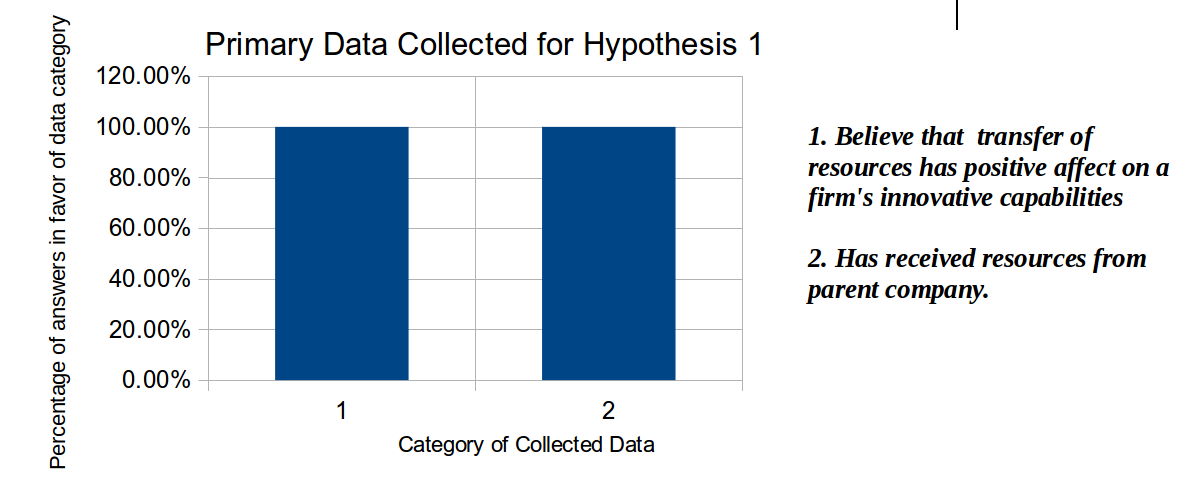
\includegraphics[width=15cm]{fig4}
	\caption{Data for Hypothesis 1}
	\label{fig4}
\end{figure}
\\
\\
Conatix CEO, David Lehrer, said the following about the resources they received
from parent company:
\\
\\
``\textbf{We received free and discounted use of office space from Humboldt University Berlin which
was valuable in the beginning, also servers and other old and used equipment from the
university}''.
\\
\\
Table \ref{table3} shows the secondary research results used for hypothesis 1.

\begin{table} [h!]
\centering
\hspace*{-1cm}
	\begin{tabular}{ |c|L{2.5cm}|L{2cm}|c|L{3cm}| } 
		\hline
		\textbf{Type of resource} & \textbf{Title} & \textbf{Authors} & \textbf{Publishing Year} & \textbf{Findings} \\
		\hline
		Research Paper & Do direct or indirect relations between incumbent firms and corporate spin-offs affect the performance of spin-offs? & Majbritt Rostgaard Evald, Ann Hojbjerg Clarke, Kent Wickstrom Jensen & 2009 & Resources received by spin-
		offs through direct or indirect
		relationships with parent firms
		help them to perform better
		than independent start-ups.
		However,
		spin-offs
		with
		indirect relations to a parent
		firm perform better than spin-offs having direct relations
		\cite{35}. \\
        \hline
        Research Paper & Whose
        child?: 
        how
        existing
        firms foster new
        firm formation  & Sierdjan Koster  & 2006 & Transfer of resources between
        firms does not always
        guarantee the success of spin-
        off. Resources lose their
        previous designations and
        position and needs to be
        managed effectively in the
        receiving firm \cite{whose_child}. \\
        \hline
	\end{tabular}
	\hspace*{-1cm}
	\caption{Secondary Research Data for Hypothesis 1}
	\label{table3}

\end{table}

\section{Data For Hypothesis 2\label{sec:data2}}
This hypothesis states that previous industry experience and managerial skills help spin-offs to
innovate better than start-ups. Questions asked to respondents for testing this hypothesis were about
previous work experience and managerial skills before joining the current organizations. Figure \ref{fig5}  shows the results of questions asked for testing Hypothesis 2.

\begin{figure}[!h]
	\centering
	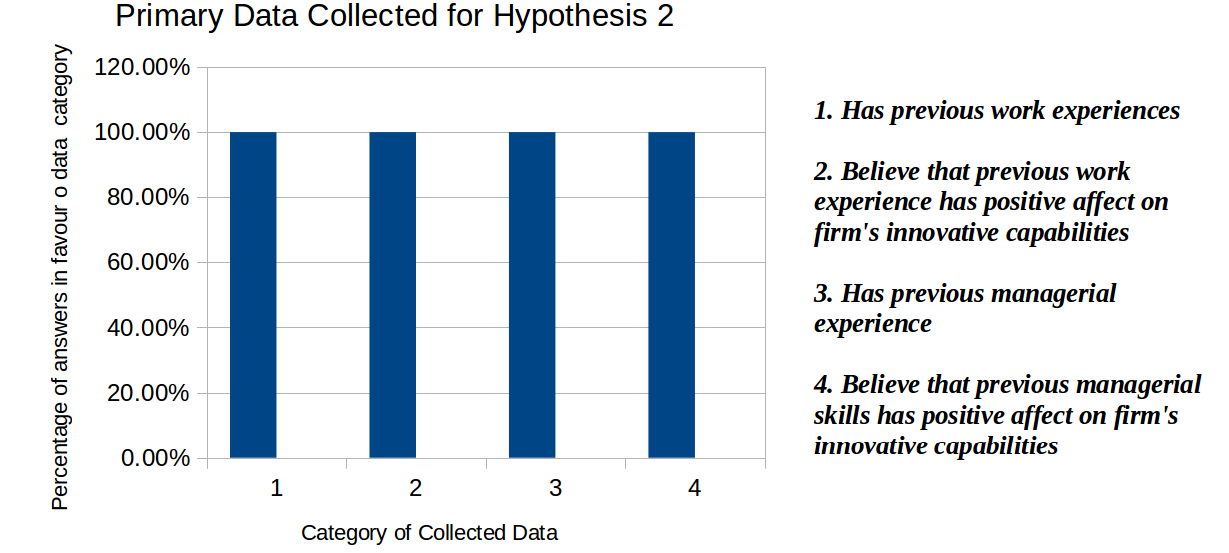
\includegraphics[width=15cm]{fig5}
	\caption{Data for Hypothesis 2}
	\label{fig5}
\end{figure}
Table \ref{table4} shows the secondary research results used for hypothesis 2.

\begin{table} [h!]
	\centering
	\hspace*{-1cm}
	\begin{tabular}{ |c|L{3cm}|L{3cm}|c|L{3cm}| } 
		\hline
		\textbf{Type of resource} & \textbf{Title} & \textbf{Authors} & \textbf{Publishing Year} & \textbf{Findings} \\
		\hline
		Research paper & The effectiveness 
		of
		university knowledge
		spillovers:
		Performance
		differences
		between
		university
		spinoffs
		and
		corporate
		spinoffs &Karl Wennberg, Johan Wiklund, Mike Wright & 2011 & Previous industry experience
		in private corporations proves to be potentially more
		valuable
		for
		spin-off
		performance in than university
		experience alone \cite{55}\\
		\hline
		Book & Success Factors 
		of
		Corporat
		Spin-Off & Alexander Tübke & 2004 & Author has described transfer
		of experience as one of the
		success factors for spin-offs.
		He has mentioned that
		managerial skills are more
		valuable
		to
		progressive
		growth of a business venture
		than technical skills. He has
		given importance to different
		types
		of
		experiences
		transferred
		in
		spin-off
		development process e.g.
		market and product related,
		technical, managerial and
		leadership \cite{57} \\
		\hline
	\end{tabular}
	\hspace*{-1cm}
	\caption{Secondary Research Data for Hypothesis 2}
	\label{table4}
\end{table}


\section{Data For Hypothesis 3\label{sec:data3}}
This hypothesis states that networking and relationships with clients and organizations help spin-
offs in their growth and progress. Questions asked to respondents for testing this hypothesis were
about previous networking with clients or other firms before starting their ventures. Figure \ref{fig6}
shows the results of questions asked for testing Hypothesis 3.

\begin{figure}[!h]
	\centering
	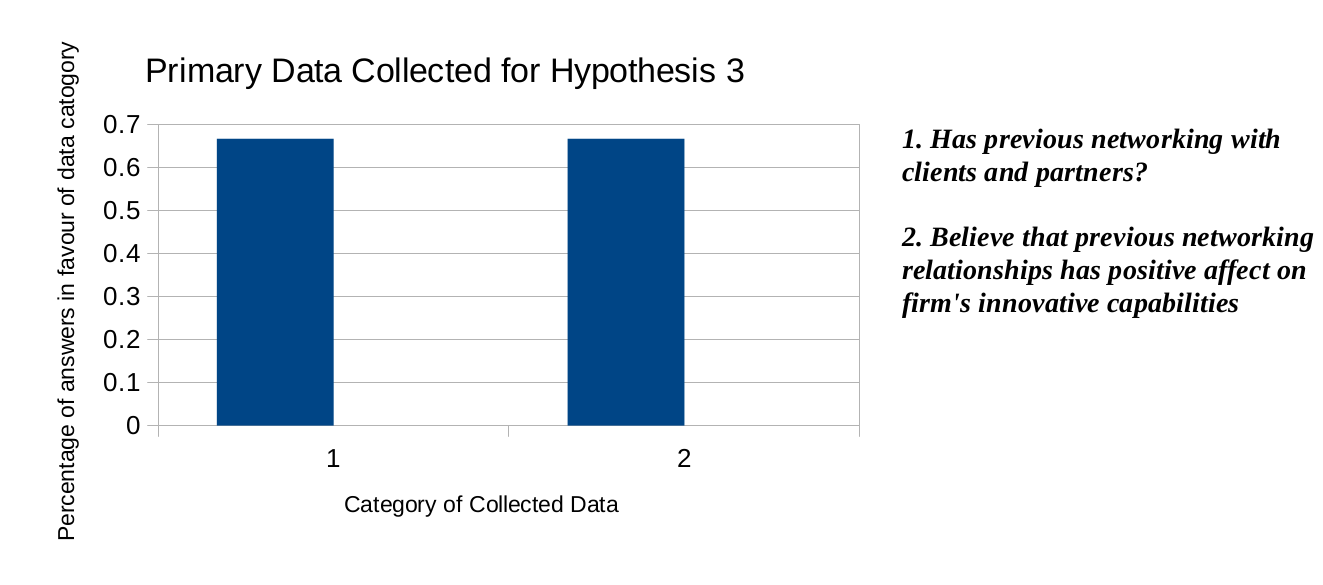
\includegraphics[width=15cm]{fig6}
	\caption{Data for Hypothesis 3}
	\label{fig6}
\end{figure}
Table \ref{table5} shows the secondary research results used for hypothesis 3.

\begin{table} [h!]
	\centering
	\hspace*{-1cm}
	\begin{tabular}{ |c|L{3cm}|L{3cm}|c|L{3cm}| } 
		\hline
		\textbf{Type of resource} & \textbf{Title} & \textbf{Authors} & \textbf{Publishing Year} & \textbf{Findings} \\
		\hline
		Research Paper & Parent company influence on spin-off performance & Tatsiana Halai & 2015 & Networking provides open
		access to potential clients,
		finances and supplies for product development. If the parent company has good
		reputation. It helps spin-offs to
		get more faith from clients
		and external relationships \cite{58}.\\
		\hline
		Research Paper & Spin-off
		firms
		and
		individual
		start-ups.
		Are
		they really
		different? &  Sierdjan Koster & 2004 & Theoretical ideas, based on
		resource theory, spin-offs
		perform better than start-ups
		based on their capabilities of
		finding ways to establish
		networks
		with
		relevant
		businesses \cite{30}. \\
		\hline
	\end{tabular}
	\hspace*{-1cm}
	\caption{Secondary Research Data for Hypothesis 3}
	\label{table5}
\end{table}
\section{Data For Hypothesis 4\label{sec:data4}}
This hypothesis states that lacking the desire and passion while joining a spin-off has bad affects on
innovation development of business. Questions asked to respondents for testing this hypothesis
were about their motivations while joining the firms. Figure \ref{fig7} shows the results of
questions asked for testing Hypothesis 4.

\begin{figure}[!h]
	\centering
	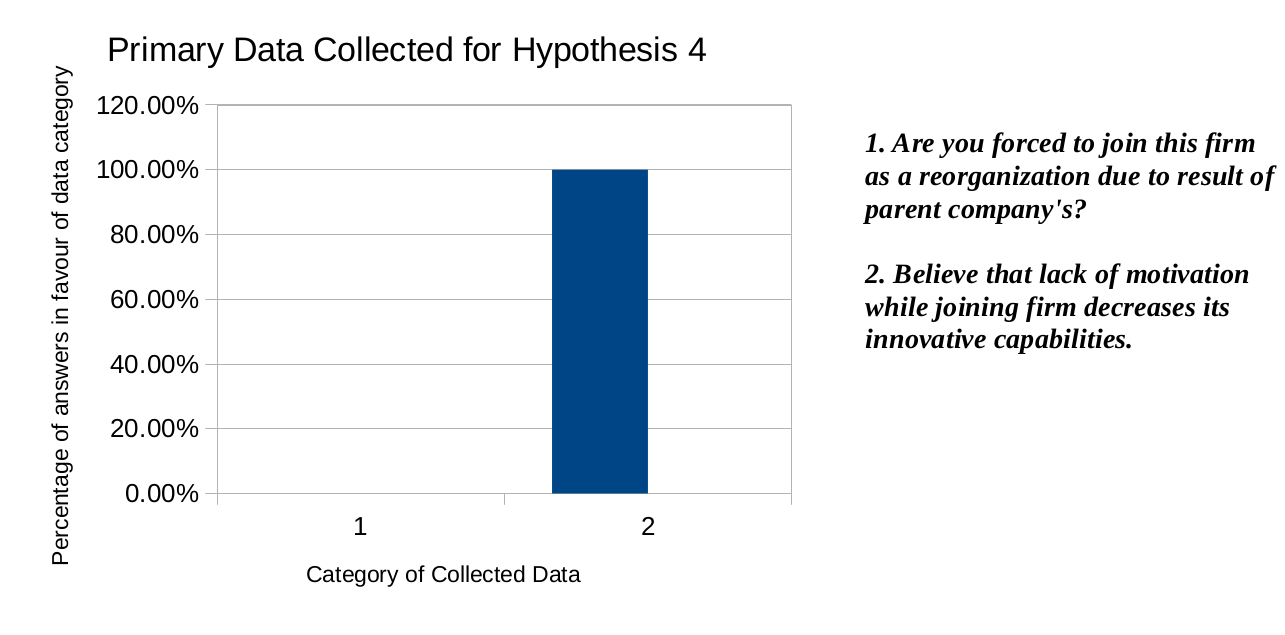
\includegraphics[width=15cm]{fig7}
	\caption{Data for Hypothesis 4}
	\label{fig7}
\end{figure}
Table \ref{table6} shows the secondary research results used for hypothesis 4.

\begin{table} [h!]
	\centering
	\hspace*{-1cm}
	\begin{tabular}{|c|L{3cm}|L{2cm}|c|L{3cm}|}
		\hline
		\textbf{Type of resource} & \textbf{Title} & \textbf{Authors} & \textbf{Publishing Year} & \textbf{Findings} \\
		\hline
		Book & A Theoretical  and Empirical Analysis, with Special Reference to Education, Second Edition & Gary S. Becker  & 1975 & Motivation is one of the major
		factors affecting productivity
		of
		employees.
		Large
		investments on human capital
		and increase in earnings
		affects employees morale
		which
		in
		turn
		affects
		company’s growth \cite{59}. \\
		\hline
		Book & Success Factors 
		of
		Corporate 
		Spin-Off & Alexander Tübke & 2004 & Author
		has
		discussed
		motivational factor as an
		important factor affecting the
		performance of spin-off. He
		has mentioned that when
		employees are forced to join
		spin-offs against their will in
		the times of parent internal
		crisis, businesses fail badly \cite{57}.\\
		\hline
	\end{tabular}
	\hspace*{-1cm}
	\caption{Secondary Research Data for Hypothesis 4}
	\label{table6}
\end{table}

    \chapter{Analysis and Results\label{cha:chapter5}}
In this section, results of primary and secondary research will be analyzed. Based on analysis,
hypotheses will be tested and results will be explained.

\section{Analysis and Findings For Hypothesis 1}
In primary research, all respondents of questionnaire agreed to the positive affects of resource
transfer on the success of spin-off. In Literature, however, some researchers believe that transferring of
resources could hinders the progress of spin-off, if not managed effectively. Some researchers have
argued that it deprived spin-off from independence and flexibility of performing operations which
negatively affected the spin-off innovation capabilities. However, majority of secondary research results are in
favor of hypothesis 1.

\section{Analysis and Findings For Hypothesis 2}
All respondents of questionnaire answered in favor of hypothesis 2. In addition, literature reviews
also supported the fact that previous industry experience and management skills help spin-offs to
outperform individual start-ups in early stages of development.

\section{Analysis and Findings For Hypothesis 3}
Two respondents (Imsys and Conatix) had previous networking relationships and believed that it
helped in innovation development. However, PTX tech GmbH, a Berlin based start-up, has no
previous connections with clients and its CEO believed that it had no affect on its innovation
capabilities. Results of secondary research are in favor of hypothesis 3. Since majority of results
support hypothesis 3, it appears that previous external relations with clients and providers help spin-offs to perform better than start-ups which do not have any networking with potential clients.


\section{Analysis and Findings For Hypothesis 4}

Both primary and secondary research support hypothesis 4. All respondents believed that lack of
motivation is a major factor affecting the progress of a firm. In literature, researchers also believe
that businesses with motivated and passionate employees flourish with bright colors.
    \chapter{Conclusion}
Main purpose of this research was to investigate the differences between innovation capabilities of
spin-offs and start-ups. In order to achieve goal of this study, hypotheses were developed regarding
major factors affecting innovation capabilities of spin-offs and start-ups. Four major factors were
chosen using literary theories which are resource-based theory, human capital theory, social capital
theory and motivational theory. In order to test hypotheses, qualitative methodology is used.
Questionnaire was being sent to three respondents which hold administrative and managerial positions in the
spin-offs and start-ups. For secondary research, books and research papers were consulted. The
results showed that transfer of resources from parent companies, previous industry experience,
management skills and networking relations help spin-offs to perform better than individual start-ups.However, spin-offs which are developed as a result of adverse affects and inefficient driving
forces in parent companies, cause lack of motivation in employees which badly affects
performance.

\section{Potential Benefits}
The conclusion of this research will help future researchers in comparative studies of spin-offs and
start-ups. It will help to further investigate the factors affecting innovation capabilities of firms.
Moreover, it can be useful to business owners for understanding the reasons for success and failures
of firms ,develop strategies for innovation development and evaluate main
challenges on road of success.
\section{Future Work}
This research can be used for future investigation of important factors impacting
the development of innovation activities of firms. More in-depth investigation and interviews can be conducted
to make the results of this study more reliable. For future work, it would be very interesting to investigate
factors impacting innovation of spin-offs and start-ups in different countries and in different development stages
of firms.


% ---------------------------------------------------------------
\backmatter % no page numbering from here
		
		% if you want to provide a glossary with explanations of important terms put it in here

    \bibliographystyle{ieeetr}
    \bibliography{./bib/references}
    
    \addchap{Annex}

\begin{appendix}

\lstset{language=,caption=Sourcecode Listing,captionpos=b,
label=yahoowidgetkon,showstringspaces=false,
basicstyle={\fontfamily{pcr}\selectfont\footnotesize}}
\begin{lstlisting}
<?xml version="1.0" encoding="UTF-8"?>
<widget>
	 <debug>off</debug>
	 <window name="myWindow" title="Hello Widget" visible="true">
		 <height>120</height>
		 <width>320</width>
		 <image src="Resources/orangebg.png">
			<name>orangebg</name>
			<hOffset>0</hOffset>
			<vOffset>0</vOffset>
		</image>
		 <text>
			 <name>myText</name>
			 <data>Hello Widget</data>
			 <color>#000000</color>
			 <size>20</size>
			 <vOffset>50</vOffset>
			 <hOffset>120</hOffset>
		 </text>
	</window>
</widget>
\end{lstlisting}

\newpage


\lstset{caption=SIP request and response packet\cite{SIPBook},
captionpos=b,label=sippacket,showstringspaces=false,
basicstyle={\fontfamily{pcr}\selectfont\footnotesize}}
\begin{lstlisting}
INVITE sip:bob@network.org SIP/2.0
Via: SIP/2.0/UDP 100.101.102.103:5060;branch=z9hG4bKmp17a
Max-Forwards: 70
To: Bob <sip:bob@network.org>
From: Alice <sip:alice@ims-network.org>;tag=42
Call-ID: 10@100.101.102.103
CSeq: 1 INVITE
Subject: How are you?
Contact: <sip:xyz@network.org>
Content-Type: application/sdp
Content-Length: 159
v=0
o=alice 2890844526 2890844526 IN IP4 100.101.102.103
s=Phone Call
t=0 0
c=IN IP4 100.101.102.103
m=audio 49170 RTP/AVP 0
a=rtpmap:0 PCMU/8000

SIP/2.0 200 OK
Via: SIP/2.0/UDP proxy.network.org:5060;branch=z9hG4bK83842.1
;received=100.101.102.105
Via: SIP/2.0/UDP 100.101.102.103:5060;branch=z9hG4bKmp17a
To: Bob <sip:bob@network.org>;tag=314159
From: Alice <sip:alice@network.org>;tag=42
Call-ID: 10@100.101.102.103
CSeq: 1 INVITE
Contact: <sip:foo@network.org>
Content-Type: application/sdp
Content-Length: 159
v=0
o=bob 2890844526 2890844526 IN IP4 200.201.202.203
s=Phone Call
c=IN IP4 200.201.202.203
t=0 0
m=audio 49172 RTP/AVP 0
a=rtpmap:0 PCMU/8000
\end{lstlisting}


\end{appendix}

\endinput


\end{document}
